% This file was created by matlab2tikz.
%
%The latest updates can be retrieved from
%  http://www.mathworks.com/matlabcentral/fileexchange/22022-matlab2tikz-matlab2tikz
%where you can also make suggestions and rate matlab2tikz.
%

\documentclass[pt]{standalone}
\usepackage{amsmath}
\usepackage{graphicx}
\usepackage[pdf]{pstricks}
\usepackage{pgfplots}
\pgfplotsset{compat=newest}
\usepgfplotslibrary{fillbetween}
%% the following commands are needed for some matlab2tikz features
\usetikzlibrary{plotmarks}
\usetikzlibrary{arrows.meta}
\usepgfplotslibrary{patchplots}
\usetikzlibrary{decorations.text}
\usetikzlibrary{shapes.multipart}
%\usetikzlibrary{external}
%\tikzexternalize % activate!

\begin{document}
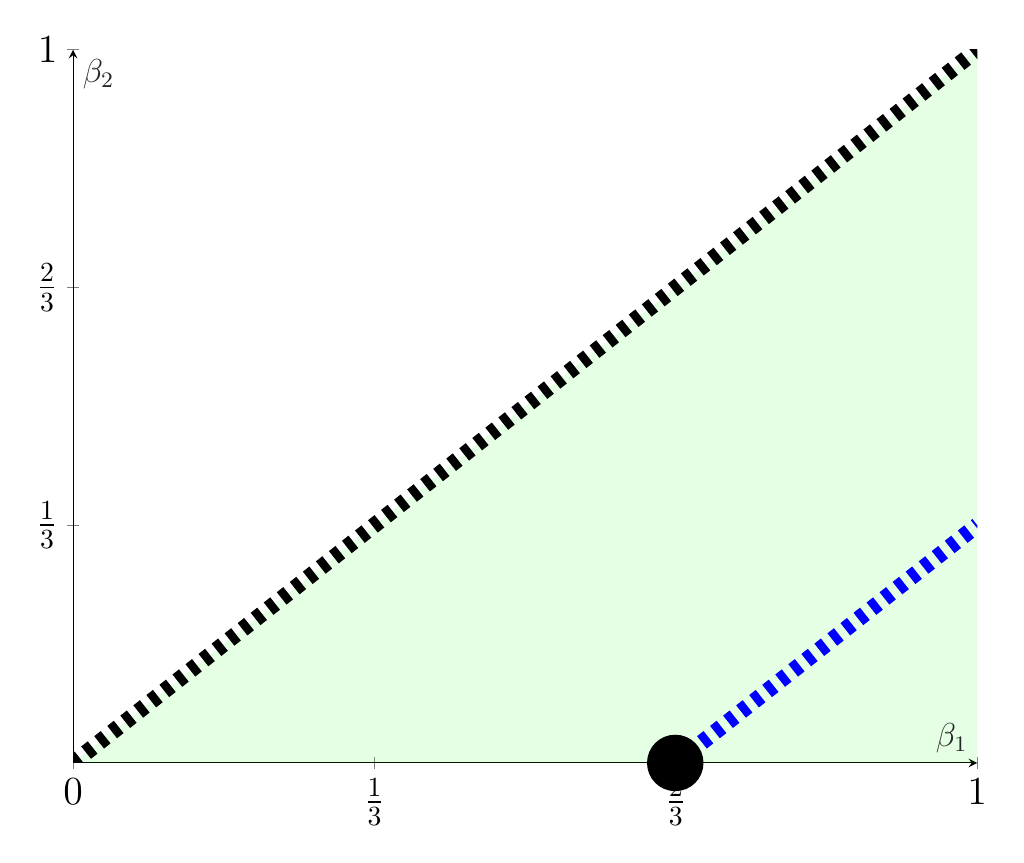
\begin{tikzpicture}[every text node part/.style={align=center}]
\tikzstyle{every node}=[font=\Large]
\begin{axis}[%
width=4.521in,
height=3.566in,
enlarge x limits=true,
enlarge y limits=true,
clip=true,
axis x line=bottom, 
axis y line=left,
at={(0.758in,0.481in)},
scale only axis,
axis x line = middle,
axis y line = middle,
xmin=0,
xmax=1,
xtick={-0.66666,-0.33333,0.33333,0.66666,1},
xticklabels = {$-\frac23$,$-\frac13$,$\frac13$,$\frac23$,$1$},
extra x ticks={0},
xlabel style={font=\color{white!15!black}},
xlabel={\large $\beta_1$},
ymin=0,
ymax=1,
ytick={0.33333,0.66666,1},
yticklabels = {$\frac13$,$\frac23$,$1$,$\frac43$},
ylabel style={font=\color{white!15!black}},
ylabel={\large $\beta_2$},
axis background/.style={fill=white},
];
\addplot+[name path=Above,mark=none, draw=none] coordinates {(-3,1) (-10,1)};

\draw[dashed,black,line width=0.2cm] (0,0) --   (1,1) ;

\draw[-,blue,line width=0.2cm,dashed] (2/3,0) --   (1,1/3) ;


\path[name path=Critical ] (0,0) -- (1,1) ;

\addplot+[name path=Below,mark=none, draw=none] coordinates {(-2,0) (2,0)};


\addplot[green,opacity=0.1] fill between[of=Critical and Below];

\addplot[mark=*,black,mark size=10pt] coordinates {(0.666,0)};

%\addplot[mark=*,blue] coordinates {(0.666,0)};
%
%\addplot[mark=*,red] coordinates {(0.8,0.133333)};



%
%\node[rotate = 60] at (axis cs: 0.3,.55) {Region 1 - \\ Trailing Dispersive Waves };
%\node[rotate = 60] at (axis cs: -0.5,0.5) {Region 2 - \\ Advancing Dispersive Waves};
%
%\draw[<->,red,ultra thick] (0,0) --   (0.8,0.8) ;
%
%\addplot[draw=none,blue,decoration={text along path,
%	text={|\Large| iSGN},
%	raise=-3ex,
%	text color={red},
%	text align={left indent={0.4\dimexpr\pgfdecoratedpathlength\relax}}},
%postaction={decorate}]
%coordinates {(0,0) (1,1)};
%
%\draw[<->,green!60!black,ultra thick] (-0.6666,0) --   (0,0) ;
%
%\addplot[draw=none,decoration={text along path,
%	text={|\Large| SGN To SWWE},
%	raise=1ex,
%	text color={green!60!black},
%	text align={left indent={0.05\dimexpr\pgfdecoratedpathlength\relax}}},
%postaction={decorate}]
%coordinates {(-0.6666,0) (0,0)};
%
%\node[] at (axis cs: 0.13,0.025) {SGN};
%\node[] at (axis cs: 0.57,0.13) {iSGN Member ($\beta_1 = \frac{2}{15}$)};
%
%\addplot[only marks] coordinates {(0,0) (-0.6666,0) (0.133333,0.133333)};
%\node[rotate=-80] at (axis cs: -0.73,0.09) {SWWE};


\end{axis}

\end{tikzpicture}%

\end{document}